\chapter{Experiments, Results and Discussions}
\label{chap:exp}
\framebox{REVIEW1}
\framebox{TODO:general introduction to the experiments}
\section{Onset Deviation Normalization}
\framebox{TODO:onset diviation problem review}
\framebox{TODO:onset diviation features plot}
\framebox{TODO:failed is excluded}

\section{Parameter Selection}
\subsection{SVM-related Parameters}
Since SVM-HMM is a combination of SVM and HMM, there are many parameters which needs adjustment from both model. Two parameters are tested to find their optimal value: the termination accuracy $\epsilon$ and the misclassification penalty factor C in SVM. Because the algorithm is an iterative one, the $\epsilon$ parameter defines the desired accuracy required for the algorithm to terminate. A smaller $\epsilon$ will result in higher accuracy, but increased execution time (because of more iterations run.) The C parameter determines how hard non-separable samples should be penalised. A large C will sacrifice larger margin for lower misclassification error, but it will make the execution longer.%Therefore, we will leave the rest of the parameters to their default value, and try to find the best C parameter.l

Because it is desirable to generate a performance in a style similar to the training examples, we use the whole set of Clementi's Sonatinas Op.36 from a single performer, and split them into two sets: the training set includes pieces No. 2 to No. 6, and the testing set includes piece No. 1. We train a model with the training set, and use the learned model to generate expressive performance. The computer generated expressive performance should have a similar expression to the testing set. 


%Structural Support Vector Machine has some parameters that needed to be adjusted. We will leave the others to the defaults and change the SVM C trad-off parameter in this experiment. Since three models are learned for three performance features, we have three parameters to adjust. 
%TODO default parameters

%[TODO: phrases count] phrases from [TODO:song counts] songs are used for training. Every first, fifth, and tenth phrases from each song is not included in the training sample, but used as testing samples. A three-by-three grid is layed out for three C parameters, each C takes the value of the powers of tenfrom [TODO: Cs] $10^{-5}$ to $10^4$, so [TODO: num of experiment] paramenters are tested. Then the result is validated
To measure the effectiveness of the $\epsilon$ and C parameters, the generated performance is compared to the performance recorded by the performer. Ideally, the generated performance will be very similar (in expression) to the recording. So, for every pair of the generated and recorded performances, we calculate their distance, and take the median value of all the distances for every C. Note that each performance feature has its own model, so we will be looking at a single performance feature and its C parameter at a time.  
First, the generated performance features sequence and the recorded one are normalized to a range from 0 to 1. The normalization is required because we want to tolerate linear scaling. Then the Euclidean distance of the two normalized sequence is calculated and divided by the length (in notes) of the phrase, since the phrase can have arbitrary length.


First we will fix C at 0.1 and test different $\epsilon$'s: 100, 10, 1, 0.75, 0.5 and 0.1. Then, we fix $\epsilon$ at the optimal value determined in the previous step and test 's: $10^{-3}, 10^{-2}, 10^{-1}, 0.5, 1, 5$, with other parameters set to default. And we will evaluate the optimal parameters and evaluate their execution time. For each $\epsilon$ or C, we calculate the distance between the generated pieces and recorded examples for all phrases in the testing set for each performer. And we take the median of all these distances for each $\epsilon$ or C.


%\begin{enumerate}
%	\item Are all the output samples successfully generated? (Generation may fail if the performance features are unreasonable, for example, negative onset timeing.)
%	\item Is the order of the notes preserved? Sometimes the first note is delayed too long and the second note is played too early, so the order is swaped.
%	\item Are there any extreme parameters that makes the expressive performance unnatural?
%\end{enumerate}

%The first two criterias are checked by python scripts, the last one is done by manual inspection.
%
%\framebox{TODO:train / gen corpus}
%\framebox{TODO:how to define distance}
%\framebox{TODO: range of Cs}
%\framebox{TODO: }
%
%\framebox{TODO:experiment result}
%\framebox{TODO: similarity v Cs}
%\framebox{TODO: }
%\framebox{TODO: }
%\framebox{TODO: }
\framebox{TODO: median}
The performance regeneration accuracy for various $\epsilon$'s are shown in Fig. \ref{fig:eps_accu}. And the time for various $\epsilon$'s are shown in Fig. \ref{fig:eps_time}. For $\epsilon$ value 100 and 10, the termination criteria is too generous, so the learning algorithm terminates almost immediately. Therefore, the model hardly learns anything, the output is a fixed value for any input. So we abandon the data points because the model had learned nothing. We can see that the accuracy drops slowly when $\epsilon$ becomes smaller. But after $\epsilon$ is smaller than 0.5, the accuracy doesn't drop anymore. So we will choose $\epsilon = 0.5 $ for the rest of the experiment to avoid unnecessary computations.

\begin{figure*}[tp]
   \begin{center}
      %TODO:Fig.:Example JSON code
      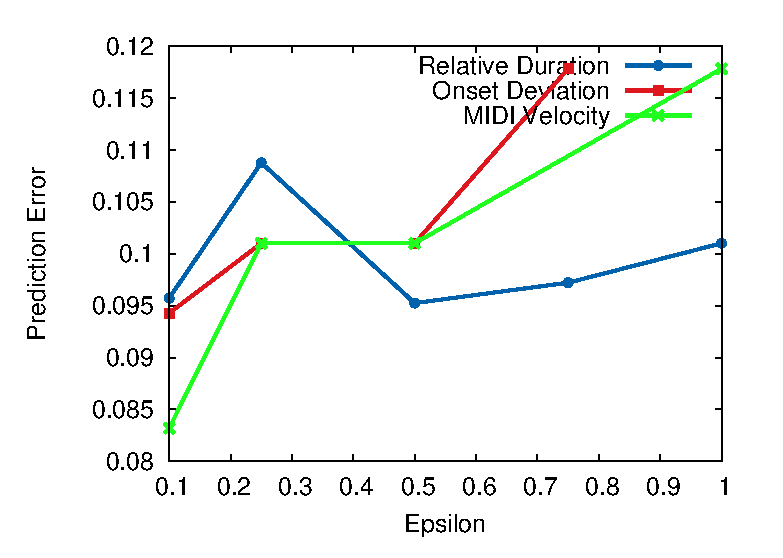
\includegraphics[width=\textwidth]{fig/eps_accu.eps}

   \end{center}
   \caption{Accuracy for Different $\epsilon$'s}
   \label{fig:eps_accu}
\end{figure*}
\begin{figure*}[tp]
   \begin{center}
      %TODO:Fig.:Example JSON code
      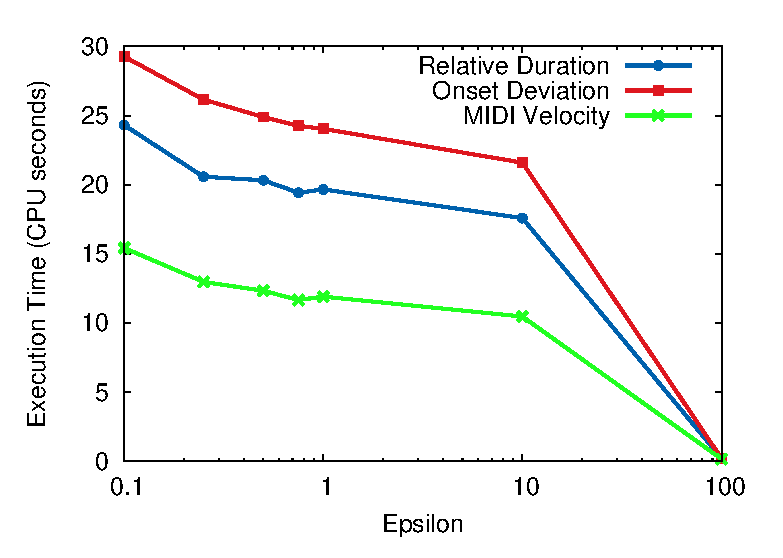
\includegraphics[width=\textwidth]{fig/eps_time.eps}

   \end{center}
   \caption{Execution Time for Different $\epsilon$'s}
   \label{fig:eps_time}
\end{figure*}
\framebox{TODO:Number of iterations}

As for different C parameter, the accuracy and execution time are shown in Fig.\ref{fig:c_accu} and Fig. \ref{fig:c_time} respectively. The accuracy forms a U shape curve, with the valley near 0.1. But the execution time grows as C goes larger, so we should choose C = 0.1 as our optimal C.

\begin{figure*}[tp]
   \begin{center}
      %TODO:Fig.:Example JSON code
      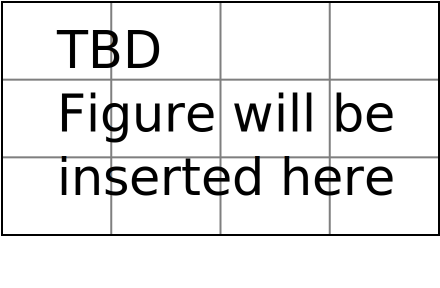
\includegraphics[width=\textwidth]{fig/TBDFigure}

   \end{center}
   \caption{Accuracy for Different C's}
   \label{fig:c_accu}
\end{figure*}
\begin{figure*}[tp]
   \begin{center}
      %TODO:Fig.:Example JSON code
      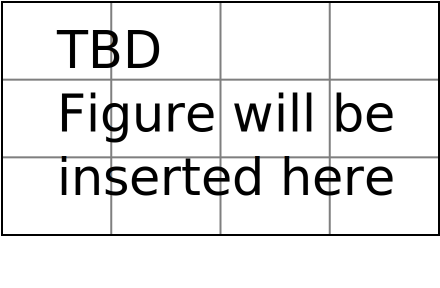
\includegraphics[width=\textwidth]{fig/TBDFigure}

   \end{center}
   \caption{Execution Time for Different C's}
   \label{fig:c_time}
\end{figure*}
\framebox{TODO:Number of iterations}
\subsection{Quantization Parameter}
\framebox{Quantization parameter time plot}

\section{Human-like Performance}
The most general purpose purpose of our expressive performance system is to create expressive, non-robotic music as oppose to vanilla MIDI. Therefore, we would like to perform a Turing-test-style survey to find out how people think about the generated expressive music.

In this survey, a computer generated expressive phrase will be compared to a human-recorded version of the same phrase. The test subject will be asked to identify which one is the computer generated one. Ideally, the computer generated phrase will be expressive enough that the subject can't effectively distinguish the generated one from the recorded one.

To generate the expressive performance phrase. We follow a six-fold cross validation pattern. For each performer in the corpus, we use all his/her recorded phrase from Clementi's Op.36 No. 2 to No. 6 to train a model. Then the model is used to generate all phrases from Clementi's Op.36 No. 1. The generate phrases are compared to the performer's recording of piece No. 1. \framebox{Maybe we should compare to other people's recording?} The process is repeated, but this time we use pieces No. 1, 3, 4, 5, 6 to train a model, and generate piece No. 2, and so on. So all six pieces will have a computer generated version and recorded version for each player's corpus.

With these music material ready, we built a survey web page to let the test subjects vote. A test subject was first asked to report their music proficiency (No music training at all, amateur or professional musician/scholar/student) and musical instrument skill. Then he/she will be asked to identify the computer generated phrase from a generated/recorded pair. Five pairs will be randomly selected from all the available pairs, and the order of appearance of the generated and recorded one will be randomized.

\framebox{All corpus vs single person}
\framebox{Turing test result}

\section{Comparing with State-of-the-Art Works}
\framebox{Discuss why state of are is not comparable}
Although we wish to compare our work with state-of-the-art works, there are some practical limitations that makes this comparison infeasible. The only place we can get formal evaluations of expressive performance systems is the RenCon contest\cite{rencon}. The most recent RenCon contest is held in 2013. The 2013 event is splitted into two main category: automatic and semi-automatic. Although the score, expressive performance audio output and votes are available, we still can't fairly compare our work with the champion of either category. First, the mandatory scores: Sonata K.466 by Domenico Scarlatti and Prelude No. 3 by Nino Rota are both polyphonic. Our system can not handle polyphonic input automatically. If we split the pieces into monophonic tracks and combine them manually, the synchronization between tracks will be totally determined by human decision, which contradicts the incentive of a automatic expressive performance system. Second, the level of automation of our work falls between the champions of the two categories, which will result in an unfair competition. The semi-automatic champion: VirtualPhilharmony by Takashi Baba et al.\cite{virtualphil}, is actually a conducting system, in which the user uses a theremin to control the musical expression. However, our system only requires the user to assign phrasing. Thus, comparing their human-controlled performance with our semi-automatic output is not fair. In the fully automatic side, however, the champion: A stochastic model of artistic deviation and its musical score for the
elucidation of performance expression by Kenta Okumura et al., doesn't require manually labeled phrasing. Therefore, our system is not on the same ground with both systems, so we decide not to compare with these systems.

There are some improvements we can make to make our work comparable to the RenCon contest results. We can loosen the semi-automatic assumption, by providing more room for human intervention. However, if we make our system more like a auxiliary system for human performance, the key evaluation criteria should not be the expressiveness of the output audio. The key performance indicator of this kind of system should be the user friendliness and the power to create highly skilled performance by unskilled amateur, which are not the goal we have in mind.

The other way is to improve our work to make it a fully automatic system. We need to implement the following capability: automatic phrasing an support polyphonic input. The first can be achieve if we employ some theories for music structures like GTTM (Generative Theory of Tonal Music)\cite{gttm}. The second can be achieved if we explicitly handles the synchronization between voices, either by machine learning or rule-based approach.



